\newcommand{\U}[1]{\ensuremath{\,\textrm{#1}}}
\newcommand{\tref}{\ensuremath{\textrm{ref}}}
\newcommand{\vthref}{\ensuremath{v_\textrm{thref}}}
\newcommand{\gkw}{\ensuremath{\texttt{GKW}}}
\newcommand{\gkdb}{\ensuremath{\texttt{GKDB}}}

\documentclass[a4paper]{report}
\usepackage{fullpage}
\usepackage{amsmath}
\usepackage{amssymb}
\usepackage{bm}
\usepackage{graphicx}
\usepackage{tabularx}
\usepackage{hyperref}
\hypersetup{plainpages=false, colorlinks=true, linkcolor=blue, citecolor=blue, urlcolor=blue, pdftitle={GKDB documentation}}

\begin{document}

\title{GKW to GKDB data conversion}

\author{Y. Camenen on behalf of the GKDB working group}

\date{Last update: June 4, 2018}

\maketitle


\tableofcontents

\chapter{Preamble}
This document describes how to transform inputs and outputs from a GKW flux-tube simulation to match the format used in the GyroKinetic DataBase (GKDB). \\ 
The reader is assumed to have some knowledge of GKW \cite{Peeters:CPC09,GKW:wiki} and to have read the documentation of the GKDB \cite{GKDB:wiki}. The structure of the present document follows that of the GKDB documentation.

\chapter{Conventions and normalisations}

\section{Coordinate systems}

In GKW, the toroidal direction is defined to have the cylindrical coordinate system $(R,Z,\varphi)$ right-handed whereas in the GKDB it is defined to have $(R,\varphi,Z)$ right-handed, see Fig.\ref{fig:coord1}. In practice, it means that: 
\begin{equation}
\varphi^\gkdb=-\varphi^\gkw
\end{equation}
\begin{figure}[h]
	\begin{center}
		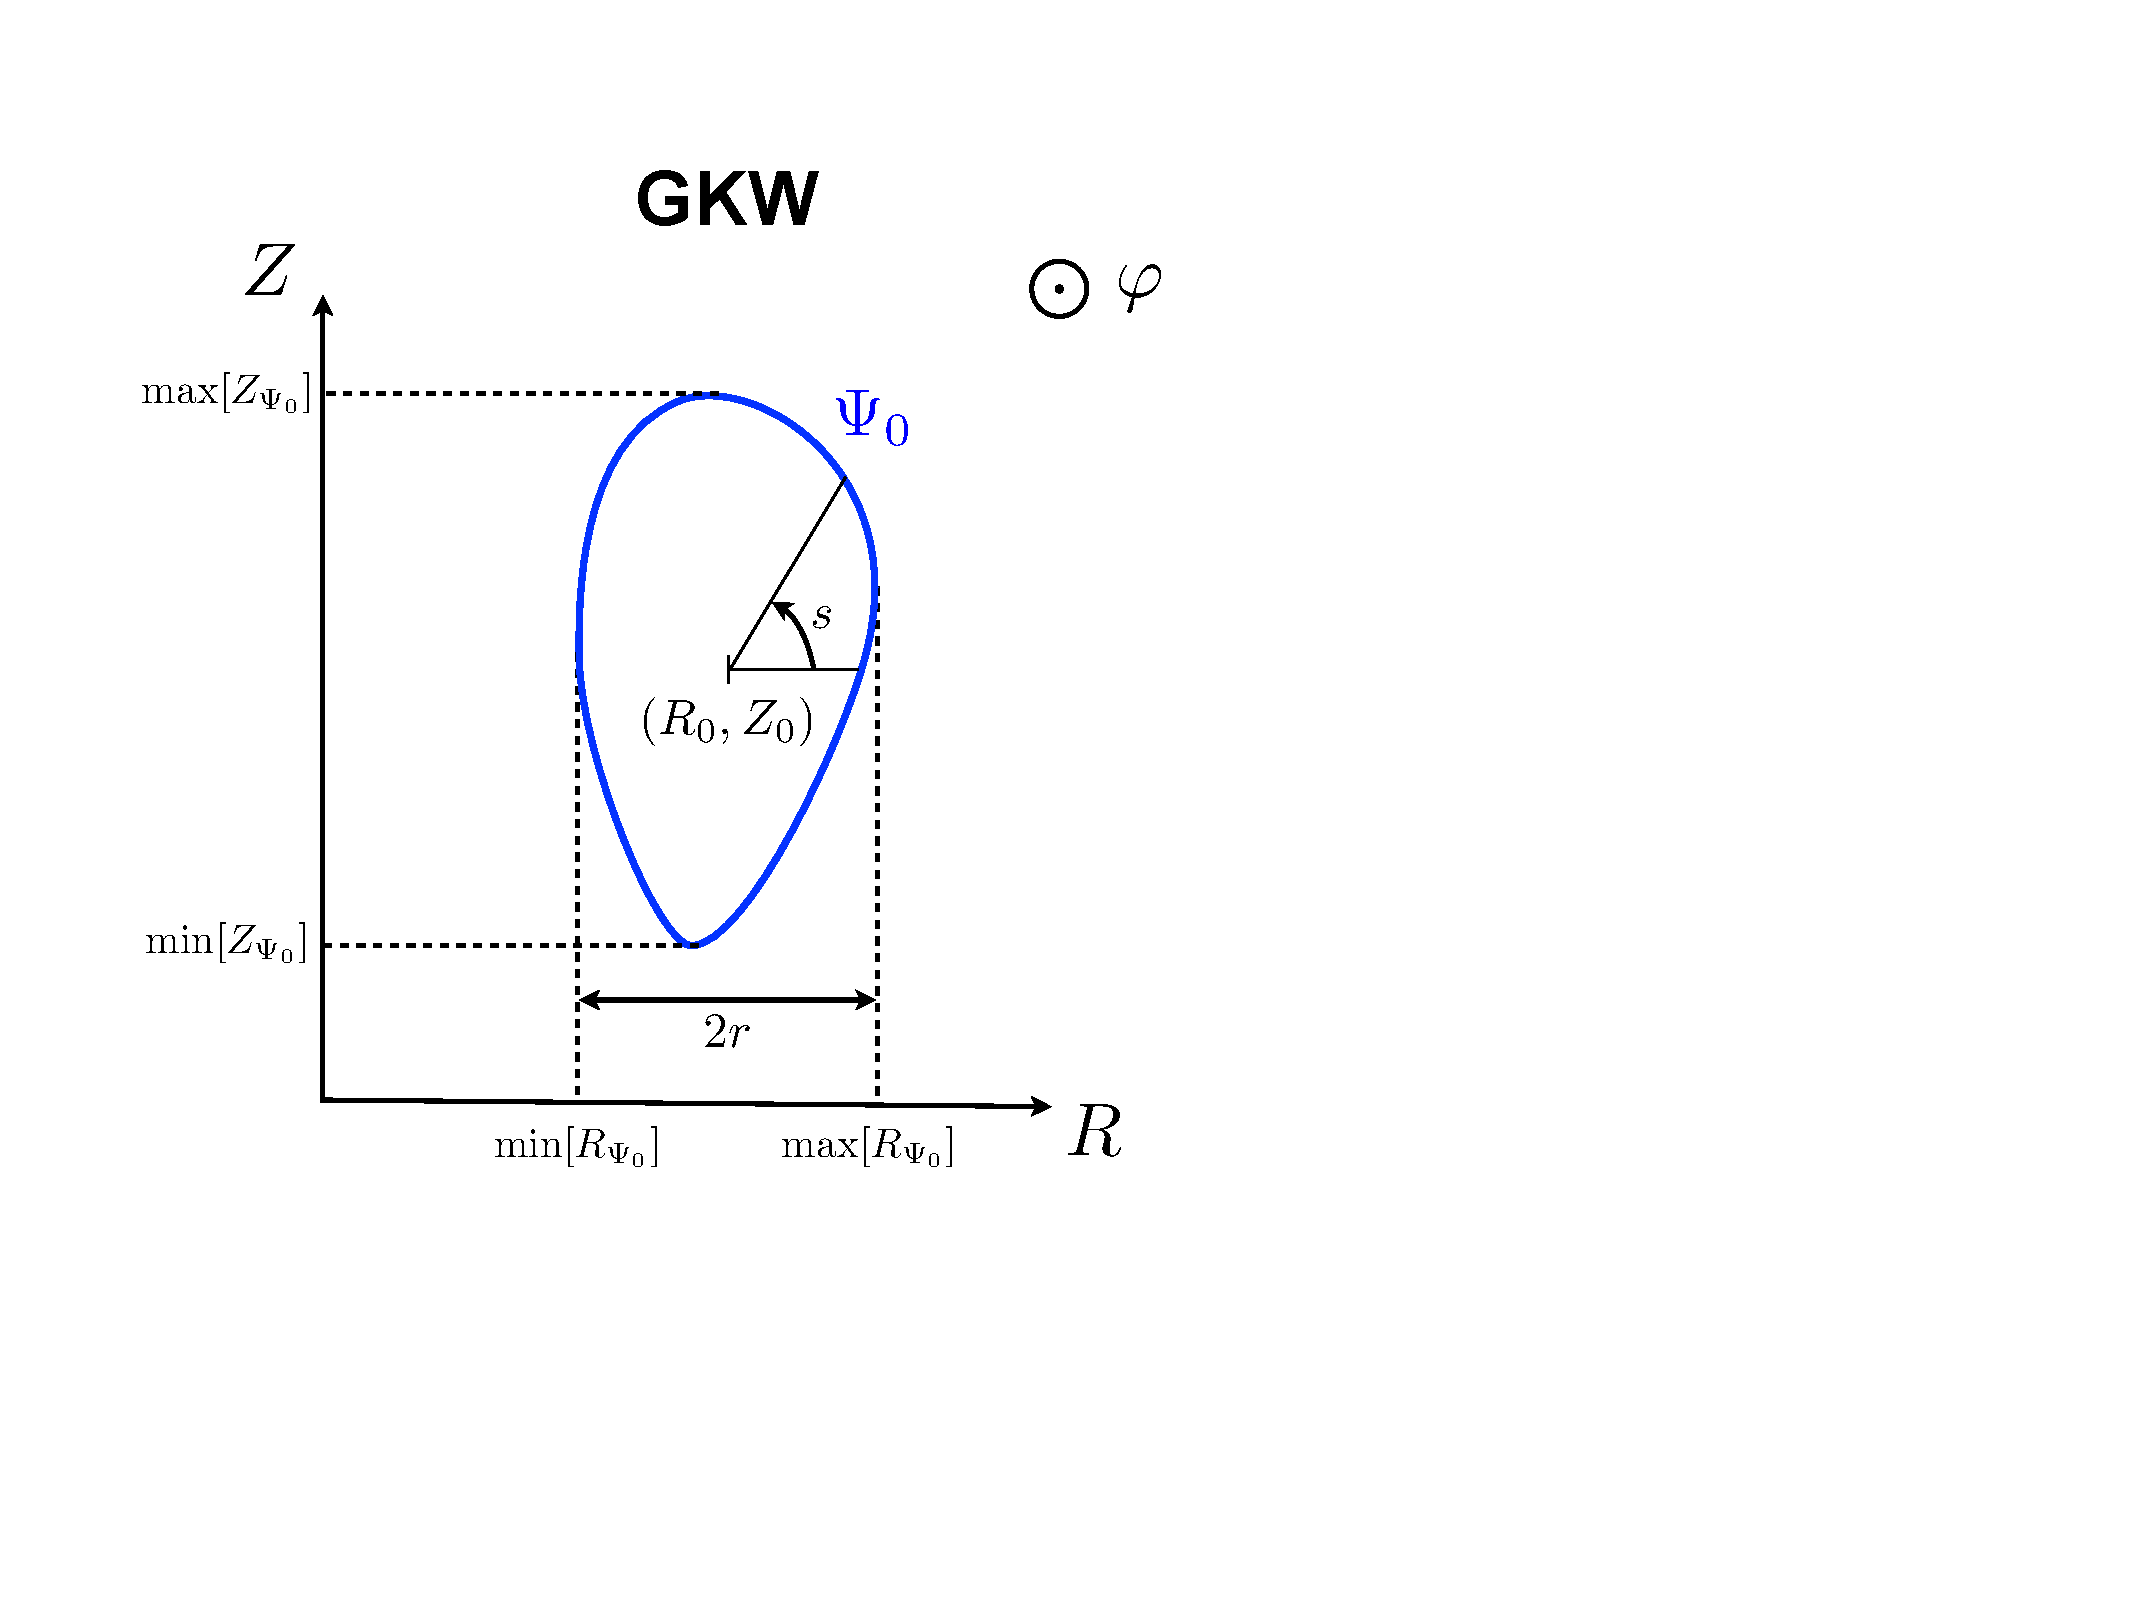
\includegraphics[width=7cm]{GKW_coord.pdf}
		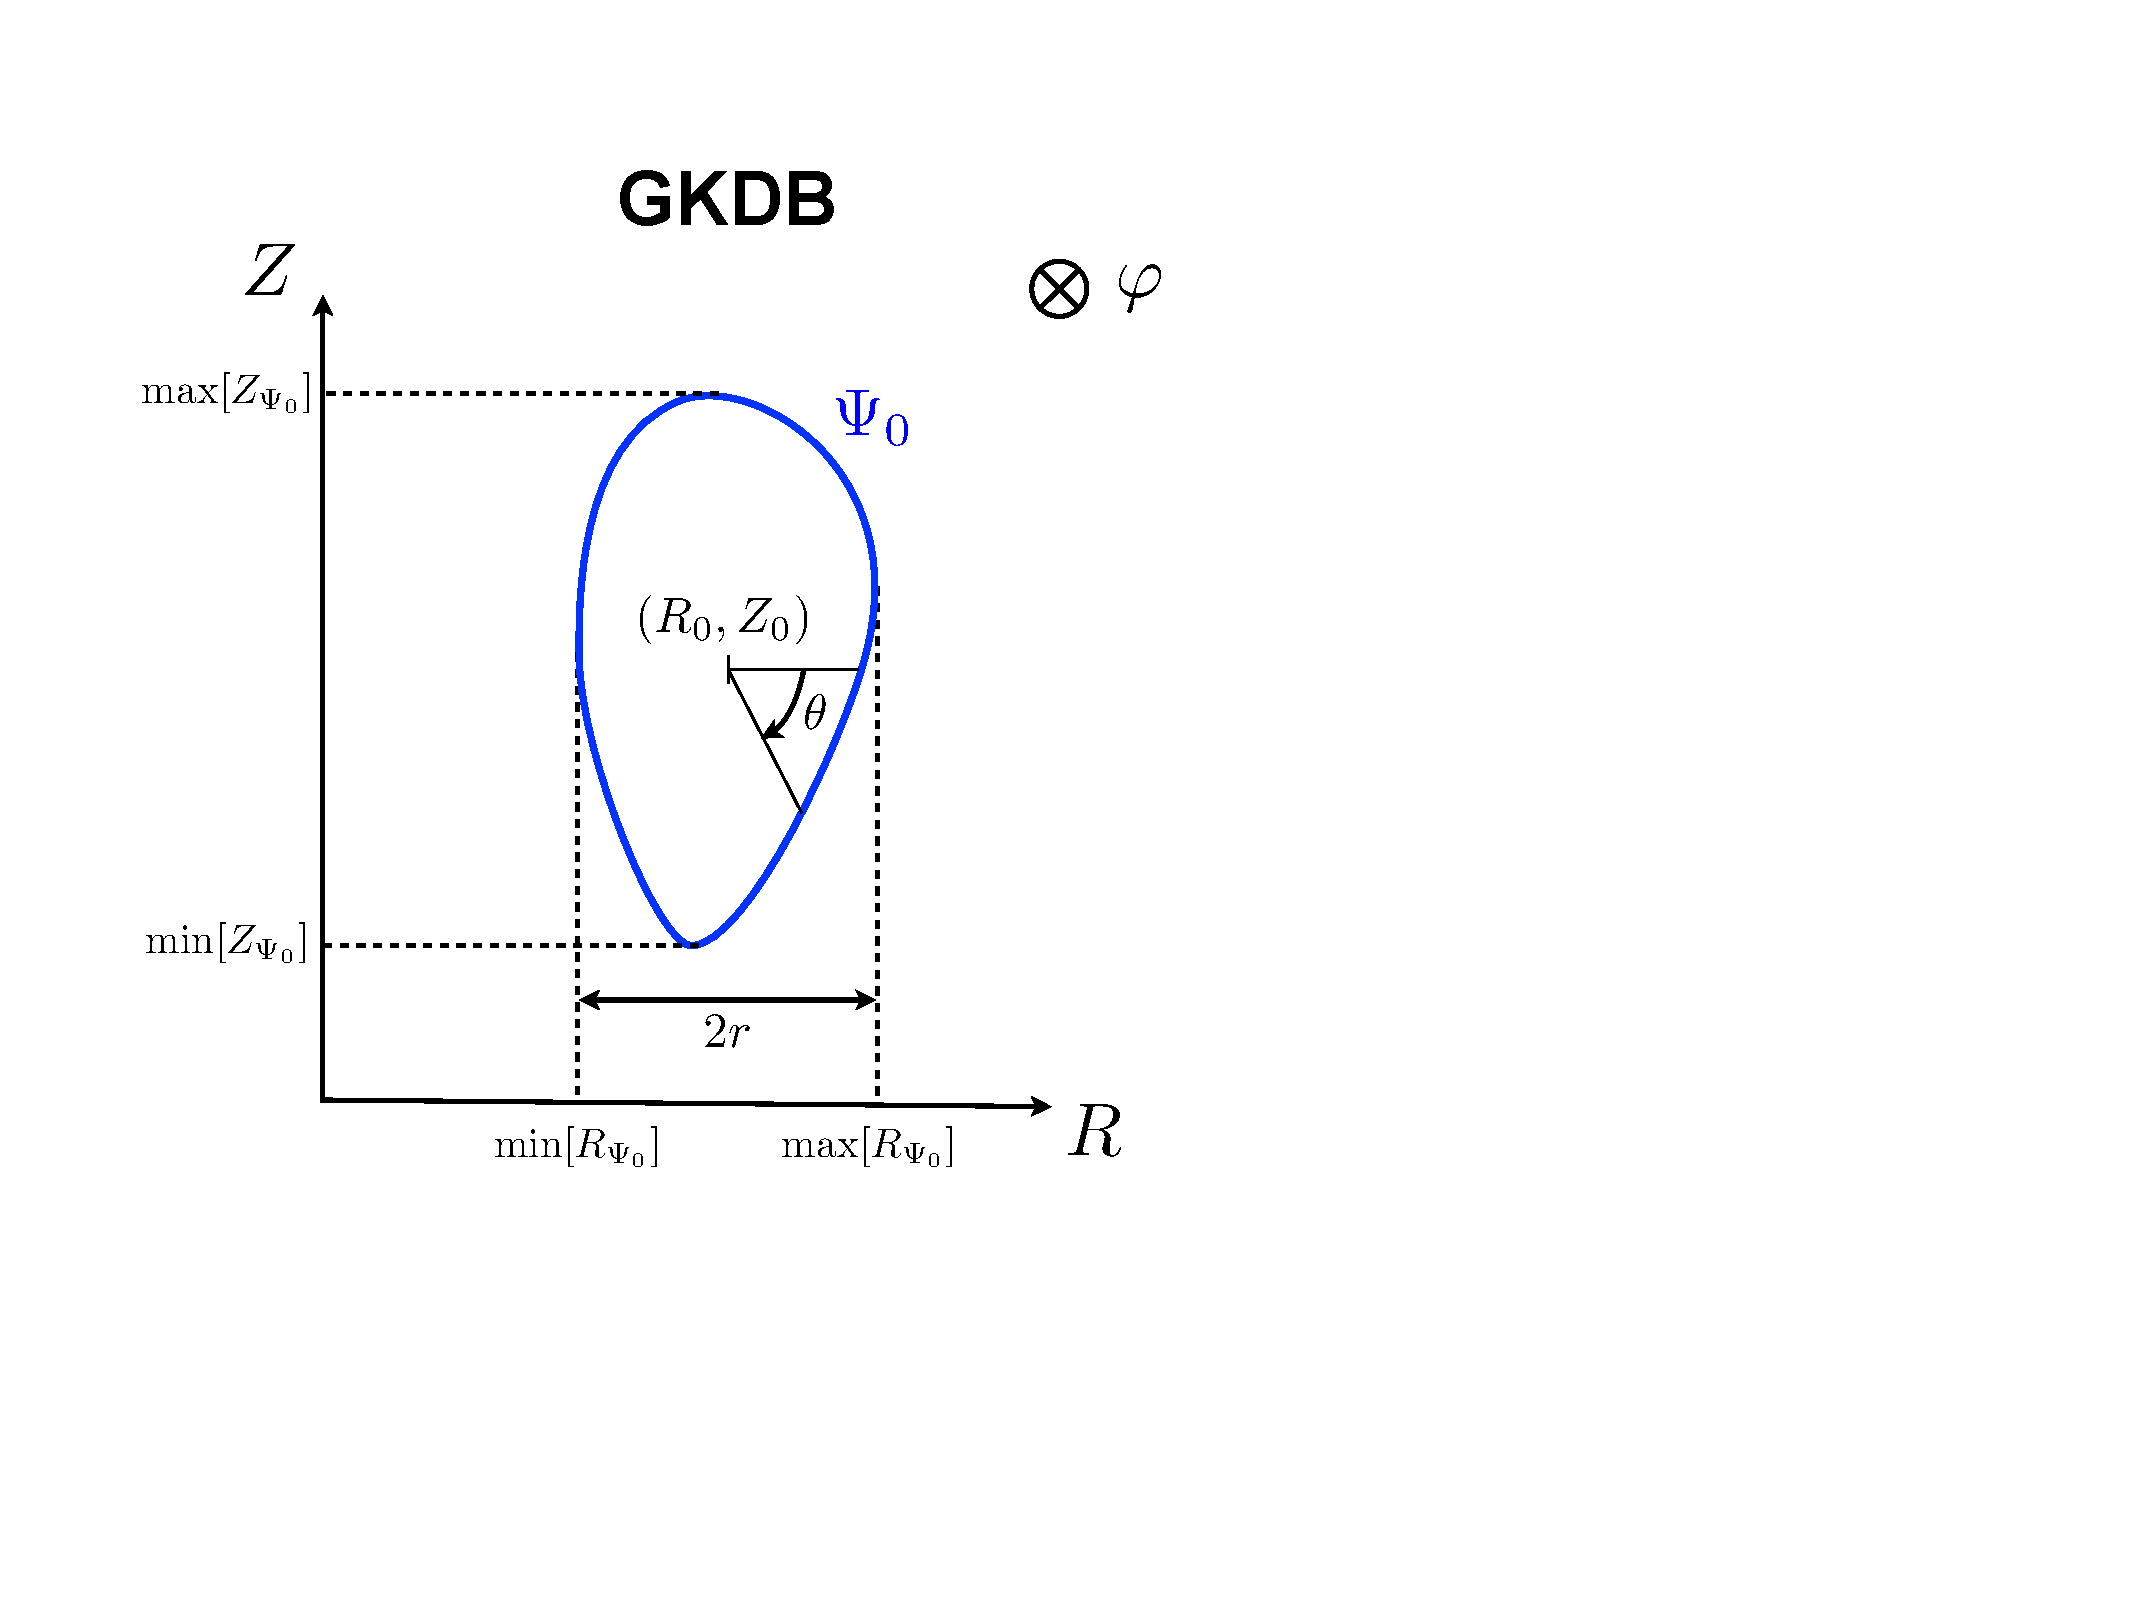
\includegraphics[width=7cm]{GKDB_coord.pdf}
		\caption{\label{fig:coord1} Cylindrical coordinate system used in GKW (left) and the GKDB (right).}
	\end{center}
\end{figure}\\
The flux surface centre definition depends on how the magnetic equilibrium is specified. For \texttt{miller} geometry, the definition of $R_0$ is identical to that used in the GKDB and $Z_0$ is given as an input in the geometry namelist:
\begin{equation}
R_0^\texttt{GKW-miller} = R_0^\gkdb \qquad \qquad Z_0^\texttt{GKW-miller} = \texttt{zmil}R_\tref^\gkw
\end{equation}
For \texttt{chease} geometry, $R_0$ is taken to be the value of \texttt{R0EXP} specified in the \texttt{hamada.dat} file and $Z_0$ is the elevation of the magnetic axis.
\begin{equation}
R_0^\texttt{GKW-chease} = \texttt{R0EXP} \qquad \qquad Z_0^\texttt{GKW-chease} = Z_\textrm{axis}
\end{equation}
The definition of the (dimensional) radial coordinate $r$ is identical in GKW and the GKDB:
\begin{equation}
r^\gkw = r^\gkdb
\end{equation}
The calculation of the  poloidal angle $\theta$ used in the GKDB from GKW inputs is documented in section~\ref{sec:magequil}. At this stage, just notice that most of the time $Z_0^\gkw\neq Z_0^\gkdb$, therefore, the points $s=0$ and $\theta=0$ do not necessarily coincide. 


\section{Reference quantities}
In GKW and the GKDB, all quantities are normalised and made dimensionless by making use of reference quantities. In what follows, normalised quantities are denoted with a "N" subscript. For instance, the normalised version of an arbitrary quantity $\mathcal{A}$ with the dimension of a length will be $\mathcal{A}_N^\gkw=\mathcal{A}/R_\tref^\gkw$ in GKW and $\mathcal{A}_N^\gkdb=\mathcal{A}/R_\tref^\gkdb$ in the GKDB. The conversion from GKW  to the GKDB  involves the ratio of reference quantities. For the example above:
\begin{equation}
\mathcal{A}_N^\gkdb = \frac{R_\tref^\gkw}{R_\tref^\gkdb} \mathcal{A}_N^\gkw
\end{equation}
The ratio of the various reference quantities used in GKW and the GKDB are:
\begin{align*}
q_\textrm{rat} &=  \frac{q_\tref^\gkw}{q_\tref^\gkdb} = - \frac{1}{\texttt{z}^\gkw_{e^-}} & R_\textrm{rat}^\texttt{miller} &= \frac{R_\tref^\texttt{GKW-miller}}{R_\tref^\gkdb} = 1 \\
m_\textrm{rat} &=  \frac{m_\tref^\gkw}{m_\tref^\gkdb} = \frac{m_e}{m_D}\frac{1}{\texttt{mass}^\gkw_{e^-}} & B_\textrm{rat}^\texttt{miller} &= \frac{B_\tref^\texttt{GKW-miller}}{B_\tref^\gkdb} = 1 \\
T_\textrm{rat} &=  \frac{T_\tref^\gkw}{T_\tref^\gkdb} = \frac{1}{\texttt{temp}^\gkw_{e^-}} &R_\textrm{rat}^\texttt{chease} &= \frac{R_\tref^\texttt{GKW-chease}}{R_\tref^\gkdb} = \frac{\texttt{R0EXP}}{R_0^\gkdb}  \\
n_\textrm{rat} &=  \frac{n_\tref^\gkw}{n_\tref^\gkdb} = \frac{1}{\texttt{dens}^\gkw_{e^-}} \frac{n_e(s=0)}{n_e(\theta=0)} & B_\textrm{rat}^\texttt{chease} &= \frac{B_\tref^\texttt{GKW-chease}}{B_\tref^\gkdb} = \frac{\texttt{B0EXP}}{B_0^\gkdb}
\end{align*}
where the $e^-$ subscript denotes the electron species and the electron to deuterium mass ratio is taken to be $\frac{m_e}{m_D}=2.7237 \times 10^{-4}$ in the GKDB.\\
The reference charge, mass, temperature and density ratio can be computed from the electron species parameters in the \texttt{SPECIES} namelist of the GKW input file. The poloidal asymmetry factor for the electron density can be computed from data in the \texttt{cfdens} file (GKW output).  With \texttt{chease} geometry, the ratios $ R_\textrm{rat}$ and $ B_\textrm{rat}$ can be computed from data in the \texttt{hamada.dat} file (GKW input).\\
The following derived quantities will also be used for the conversion:
\begin{align*}
v_\textrm{thrat} &= \sqrt{\frac{T_\textrm{rat}}{m_\textrm{rat}}} & \rho_\textrm{rat} = \frac{q_\textrm{rat} B_\textrm{rat}}{m_\textrm{rat}v_\textrm{thrat}}
\end{align*}


\chapter{Inputs}
\section{Magnetic equilibrium} \label{sec:magequil}
Only \texttt{miller} and \texttt{chease} magnetic equilibrium specifications are compatible with the GKDB format (\texttt{s-alpha} and \texttt{circ} are not an exact solution of the Grad-Shafranov equation).
\subsection{Flux surface centre}
Let's call $\{R_{\Psi_0},Z_{\Psi_0}\}$ a set of points discretizing the flux surface of interest.\\
The values of $\{R_{\Psi_0},Z_{\Psi_0}\}/R_\tref^\gkw$ are available in the \texttt{geom.dat} file (GKW output) and can be used to compute $\{R_0^\gkdb,Z_0^\gkdb\}/R_\tref^\gkw$. 

\subsection{Poloidal angle}
With these values, one can then compute the GKDB poloidal angle $\theta$:
\begin{equation}
 \tan \theta = - \frac{Z_{\Psi_0}/R_\tref^\gkw-Z_0^\gkdb/R_\tref^\gkw}{R_{\Psi_0}/R_\tref^\gkw-R_0^\gkdb/R_\tref^\gkw}
\end{equation}
As the discretisation of the flux surface in \texttt{geom.dat} is done on the GKW $s$ grid, the equation above gives the relationship between $\theta$ and $s$.

\subsection{Radial coordinate}
\begin{equation}
r_N^\gkdb = r_N^\gkw \cdot R_\textrm{rat}= \texttt{eps}\cdot R_\textrm{rat}
\end{equation}

\subsection{Toroidal field and current direction}
\begin{equation}
 s_b^\gkdb = - s_b^\gkw=-\texttt{signb} \qquad \textrm{and} \qquad s_j^\gkw=-s_j^\gkw=-\texttt{signj}
\end{equation}

\subsection{Safety factor}
\begin{equation}
q^\gkdb = s_b^\gkw s_j^\gkw q^\gkw = \texttt{signb}\cdot\texttt{signj}\cdot\texttt{q}
\end{equation}

\subsection{Magnetic shear}
\begin{equation}
\hat{s}^\gkdb = \hat{s}^\gkw = \texttt{shat}
\end{equation}

\subsection{Pressure gradient (entering the curvature drift)}
\begin{equation}
\beta^{' \gkdb}_N = - \beta^{' \gkw}_N \frac{B_\textrm{rat}^2}{R_\textrm{rat}}
\end{equation}
The value of $\beta^{' \gkw}_N $ is taken from \texttt{betaprime\_ref} for \texttt{miller} geometry or from the \texttt{geom.dat} file for \texttt{chease} geometry.

\subsection{Plasma shape}
To compute the shaping Fourier coefficients and their radial derivatives, one first need to compute:
\begin{equation}
 a_N^\gkdb(r,\theta)=\frac{1}{R_\tref^\gkdb}\sqrt{\left[R_{\Psi_0}(r,\theta)-R_0^\gkdb\right]^2 + \left[Z_{\Psi_0}(r,\theta)-Z_0^\gkdb\right]^2} 
\end{equation}
For \texttt{miller} geometry, this can be done by computing $\{R_{\Psi_0}(r,\theta),Z_{\Psi_0}(r,\theta)\}/R_\tref^\gkw$ from the Miller parameters of the GKW input files and then perform the Fourier expansion.\\
For \texttt{chease} geometry $\{R_{\Psi_0}(r,s),Z_{\Psi_0}(r,s)\}$ is directly available in the \texttt{hamada.dat} file and can be used together with the relationship between $\theta$ and $s$ to compute the Fourier coefficients. 

\section{Species}

\subsection{Charge}
\begin{equation}
Z_{sN}^\gkdb = Z_{sN}^\gkw \cdot q_\textrm{rat} = \texttt{z}_s \cdot q_\textrm{rat} 
\end{equation}

\subsection{Mass}
\begin{equation}
m_{sN}^\gkdb = m_{sN}^\gkw \cdot m_\textrm{rat} = \texttt{mass}_s \cdot m_\textrm{rat}
\end{equation}

\subsection{Density}
\begin{equation}
n_{sN}^\gkdb(\theta=0) = n_{sN}^\gkw(\theta=0) \cdot n_\textrm{rat} = \texttt{dens}_s \cdot n_\textrm{rat} \cdot \frac{n_{sN}^\gkw(\theta=0)}{n_{sN}^\gkw(s=0)}
\end{equation}
In the presence of poloidal asymmetries, the density at $\theta=0$ can be obtained from the \texttt{cfdens} output file. In this file, the first column is the $s$ grid, then comes the logarithmic density gradient for each species and finally the density for each species (all with GKW normalisations). 

\subsection{Logarithmic density gradient}
\begin{equation}
\frac{R_\tref^\gkdb}{L_{n_s}^\gkdb}(\theta=0) =  \frac{R_\tref^\gkw}{L_{n_s}^\gkw}(\theta=0) \cdot  R_\textrm{rat} = \texttt{rln}_s \cdot  R_\textrm{rat} \cdot \frac{{L_{n_s}^\gkw}(\theta=0)}{{L_{n_s}^\gkw}(s=0)}
\end{equation}
In the presence of poloidal asymmetries, the logarithmic density gradient at $\theta=0$ can be obtained from the \texttt{cfdens} output file. In this file, the first column is the $s$ grid, then comes the logarithmic density gradient for each species and finally the density for each species (all with GKW normalisations). 

\subsection{Temperature}
\begin{equation}
T_{sN}^\gkdb = T_{sN}^\gkw \cdot T_\textrm{rat} = \texttt{temp}_s \cdot T_\textrm{rat}
\end{equation}

\subsection{Logarithmic temperature gradient}
\begin{equation}
\frac{R_\tref^\gkdb}{L_{T_s}^\gkdb} =  \frac{R_\tref^\gkw}{L_{T_s}^\gkw} \cdot R_\textrm{rat} = \texttt{rlt}_s \cdot R_\textrm{rat}
\end{equation}

\subsection{Toroidal velocity}
\begin{equation}
u_N^\gkdb = s_b^\gkw\cdot u_N^\gkw \cdot \frac{v_\textrm{thrat}}{R_\textrm{rat}}  = \texttt{signb} \cdot \texttt{vcor} \cdot \frac{v_\textrm{thrat}}{R_\textrm{rat}}
\end{equation}

\subsection{Toroidal velocity gradient}
\begin{equation}
u^{'\gkdb}_{sN} = s_b^\gkw\cdot  u^{'\gkw}_{sN} \cdot \frac{v_\textrm{thrat}}{R_\textrm{rat}^2} = \texttt{signb} \cdot \texttt{uprim}_s \cdot \frac{v_\textrm{thrat}}{R_\textrm{rat}^2}
\end{equation}

\subsection{Plasma beta}
\begin{equation}
\beta_{eN}^\gkdb = \beta_N^\gkw \cdot n_\textrm{rat} \cdot T_\textrm{rat} \cdot B_\textrm{rat}^2 
\end{equation}
The value of $\beta_N^\gkw$ is either taken from the input \texttt{beta\_ref} of the \texttt{SPCGENERAL} namelist when the  \texttt{beta\_type='ref'} option is used or extracted from the output file \texttt{out} when the  \texttt{beta\_type='eq'} option is used.
 
\subsection{Collisionality}
\begin{equation}
\nu_{eN}^\gkdb = \frac{e^4}{4\pi\varepsilon_0^2}\frac{1}{q_\textrm{rat}^4}\frac{T_\textrm{rat}^2}{n_\textrm{rat}R_\textrm{rat}}\frac{n_\tref^\gkw R_\tref^\gkw}{\left.T_\tref^{\gkw}\right.^2} = \frac{e^4}{4\pi\varepsilon_0^2}\frac{1}{q_\textrm{rat}^4}\frac{T_\textrm{rat}^2}{n_\textrm{rat}R_\textrm{rat}} \frac{\texttt{nref}\cdot\texttt{rref}}{\texttt{tref}^2}
\end{equation}
Note that the expression above assumes that the \texttt{freq\_override} option is set to false. 

\subsection{Debye length}
Always zero in GKW runs.

\section{Wave vector}
\subsection{Radial wave vector}
\begin{equation}
\left. k_{r*}\rho_\tref\right.^\gkdb = \texttt{krrho}\cdot\frac{1}{\rho_\textrm{rat}}\cdot\sqrt{\frac{g^{\psi\psi}(\theta=0)}{g^{\psi\psi}(s=0)}}
\end{equation}
The quantity $g^{\psi \psi}$ is given on the $s$ grid in \texttt{geom.dat}

\subsection{Binormal wave vector}
\begin{equation}
\left. k_{\theta*}\rho_\tref\right.^\gkdb = \texttt{kthrho}\cdot\frac{1}{\rho_\textrm{rat}}\cdot\sqrt{\frac{g^{\zeta\zeta}(\theta=0)}{g^{\zeta\zeta}(s=0)}}
\end{equation}
The quantity $g^{\zeta \zeta}$ is given on the $s$ grid in \texttt{geom.dat}


\chapter{Outputs}

\section{Mode amplitude}
The normalised fields in GKW and the GKDB are related as follows:
\begin{equation}
\hat{\phi}_N^\gkdb = \hat{\phi}_N^\gkw\cdot\frac{T_\textrm{rat}\rho_\textrm{rat}}{q_\textrm{rat}R_\textrm{rat}}, \qquad \qquad
\hat{A}_{\parallel N}^\gkdb = \hat{A}_{\parallel N}^\gkw\cdot\frac{B_\textrm{rat}\rho_\textrm{rat}^2}{R_\textrm{rat}}, \qquad \qquad 
\hat{B}_{\parallel N}^\gkdb = \hat{B}_{\parallel N}^\gkw\cdot\frac{B_\textrm{rat}\rho_\textrm{rat}}{R_\textrm{rat}},  
\end{equation}
In GKW linear runs, the exponentially growing fields are further normalised with respect to the mode amplitude:
\begin{equation}
\hat{\phi}_{NN}^\gkw = \frac{1}{\mathcal{A}_f^\gkw}\hat{\phi}_N^\gkw,  \qquad \qquad \hat{A_\parallel}_{NN}^\gkw = \frac{1}{\mathcal{A}_f^\gkw}\hat{A_\parallel}_N^\gkw,  \qquad \qquad \hat{B_\parallel}_{NN}^\gkw = \frac{1}{\mathcal{A}_f^\gkw}\hat{B_\parallel}_N^\gkw
\end{equation}
with
\begin{equation}
\mathcal{A}_f^\gkw = \sqrt{\int \left[|\hat{\phi}_N^\gkw|^2 + |\hat{A}_{\parallel N}^\gkw|^2+|\hat{B}_{\parallel N}^\gkw|^2\right] \,\textrm{d}s} \bigg/ \int \,\textrm{d}s
\end{equation}
The mode amplitude used to normalise linear runs and compute the mode growth rate in the GKDB is 
\begin{equation}
\mathcal{A}_f^\gkdb  = \sqrt{\frac{1}{2\pi}\left.\int \left[|\hat{\phi}_N^\gkdb|^2 + |\hat{A}_{\parallel N}^\gkdb|^2  + |\hat{B}_{\parallel N}^\gkdb|^2\right] \,\textrm{d}\theta \right.}
\end{equation}
and the ratio of the GKDB to GKW mode amplitudes is therefore given by:
\begin{equation}
\frac{1}{\mathcal{A}_\textrm{rat}} = \frac{\mathcal{A}_f^\gkdb}{\mathcal{A}_f^\gkw} = \sqrt{\frac{1}{2\pi}\left[ |\frac{T_\textrm{rat}\rho_\textrm{rat}}{q_\textrm{rat}R_\textrm{rat}}\cdot\hat{\phi}_{NN}^\gkw|^2 + |\frac{B_\textrm{rat}\rho_\textrm{rat}^2}{R_\textrm{rat}}\cdot\hat{A}_{\parallel NN}^\gkw|^2+|\frac{B_\textrm{rat}\rho_\textrm{rat}}{R_\textrm{rat}}\cdot\hat{B}_{\parallel NN}^\gkw|^2\right]\,\textrm{d}\theta }
\end{equation}
The mode amplitude ratio can therefore be computed from the GKW output file \texttt{parallel.dat} which contains $\hat{\phi}_{NN}^\gkw(s)$, $\hat{A_\parallel}_{NN}^\gkw(s)$ and $\hat{B_\parallel}_{NN}^\gkw(s)$. Note that in this file, the fields may have been rotated in the complex plane, but this does not impact the mode amplitude calculation.

\section{Mode growth rate and frequency}


\bibliographystyle{unsrt}
\bibliography{gkw2gkdb}

\end{document}
